\documentclass[11pt,letterpaper]{report}

\usepackage[utf8]{inputenc}
\usepackage[english]{babel}
\usepackage[english]{isodate}
\usepackage[parfill]{parskip}
\usepackage{graphicx}
\usepackage{subfigure}
%\usepackage[hidelinks]{hyperref}
\usepackage{hyperref}

\usepackage{sstmanual}

\addtolength{\oddsidemargin}{-.75in}
\addtolength{\evensidemargin}{-.75in}
\addtolength{\textwidth}{1.5in}

\addtolength{\topmargin}{-.75in}
\addtolength{\textheight}{1.5in}

\setcounter{secnumdepth}{2}
\setcounter{tocdepth}{4} % show paragraphs in TOC

\title{SST Core Python Module Manual}
\date{\today}

\begin{document}
\maketitle
\newpage

\pagenumbering{Roman}

\begingroup
  \hypersetup{hidelinks}
  \tableofcontents
\endgroup
\newpage
%\listoffigures
%\newpage
%\listoftables
%\newpage
\pagenumbering{arabic}

\chapter{Introduction}

SST provides a python module to allow interaction with the simulation
build system.  This python module is used in the input python script
for the purpose of building the graph that represents the simulation
to be performed.  This is done by providing class and functions to
define the elements of the simulation, their parameters, and how they
are interconnected.  The user can also optionally enable statistics
and create a user specified partitioning for the described model.
Behind the scenes, these classes will build the c++ data structure
that is used by SST to construct the simulation model.

The SST core python module is defined in cpython and is only
available in the python interpreter launched within a running SST
executable.  The module is accessed by importing the sst module.  This
can be done in a number of ways.  The two most common being:

\begin{pycodeexample}{}
# Import SST python module using sst. prefix
import sst
# Import SST python module members into current namespace
from sst import *
\end{pycodeexample}

Within this module, there are a number of available classes and global
functions.  The available classes are: Component, SubComponent, Link,
StatisticOutput and StatisticGroup.  The global functions are divided
between general functions and functions operating on or returning one
of the available objects.  This document will first discuss the
available classes in the SST python module and will then document the
global functions.


\chapter{SST Python Classes}

There are 5 classes available in SST: Component, SubComponent, Link,
StatisticGroup and StatisticOutput.  The Component and SubComponent
classes share many of the same functions and will be covered together.

\section{Component/SubComponent Classes}

The Component and SubComponent python classes represent the Component
and SubComponent C++ classes that are used to implement the simulation
models used in SST.  They are similar, and have similar APIs, but
SubComponents can only exist inside of Components.  Subsequently,
Components are instanced directly, but SubComponents are only
instanced through a Component or another SubComponent.


Figure~\ref{fig:component-structure} shows the main pieces of the
Component/SubComponent.

\begin{figure}[h]
  \centering
  \subfigure[Main structures of the Component and SubComponent objects]{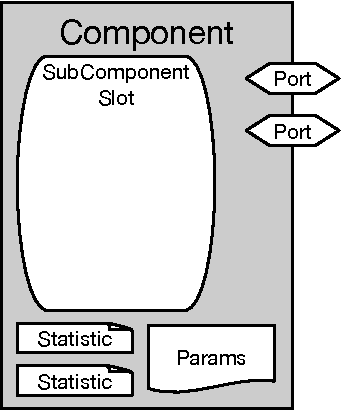
\includegraphics[width=0.3\textwidth]{figures/component-structure.pdf}} \hspace{1in}
  \subfigure[Component with SubComponents loaded, showing that SubComponents can be arbitrarily nested]{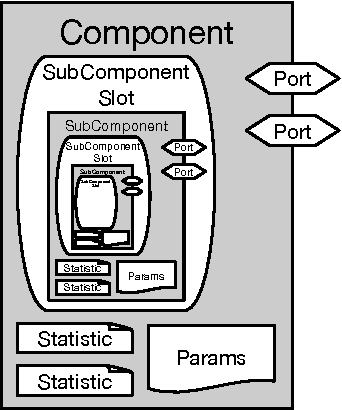
\includegraphics[width=0.3\textwidth]{figures/component-structure-with-subcomponent.pdf}}
  \caption[Structure of a Component]{Structure of a Component}
  \label{fig:component-structure}
\end{figure}

An instance of Component is created using:


\begin{functiondoc}{Component(name, element_type)}
  {Creates a new Component object.}

  \param{name} (type: string) name of the Component specified as
  string.  The name can be used to get a handle to the Component later
  in the python code.  The name is also available to the c++
  implementation of the Component

  \param{element\_type} (type: string) type of the Component in the
  lib.element format (for example, merlin.hr\_router) specified as a
  string

  \returns{Component object}
\end{functiondoc}

A SubComponent is created by calling setSubComponent() on either a
Component or SubComponent object.  Instancing a SubComponent in this
way creates a User SubComponent and allows the user to specify the
parameters and statistics directly on the SubComponent.  The name of
the SubComponent is automatically generated using the name of the
parent Component and the slot\_name(s) in which SubComponents are
loaded.  If more than one SubComponent is loaded into a slot, the
slot\_name is also indexed using square brackets (e.g. [0]).  This
name can be used to get a handle to the SubComponent later in the
python code.  See setSubComponent function description below.


\begin{functiondoc}{setSubComponent(slot_name, element_type, slot_index = 0)}
  { Inserts a SubComponent of the specified type into the indicated
    slot name and index and creates a new SubComponent object }

  \param{slot_name} (type: string) name of the slot in which the
  SubComponent should be loaded.

  \param{element_type} type of the SubComponent in the lib.element
  format (for example, merlin.linkcontrol)

  \param{slot_index} (type: string) slot index in which the
  SubComponent should be inserted.  This defaults to 0 and is not
  required if only one SubComponent is being loaded into the specified
  slot.  Each SubComponent must be loaded into a unique slot\_index
  and some (Sub)Components will require the indexes to be linear with
  no gaps.

  \returns{SubComponent object}
\end{functiondoc}


\subsection{Functions Common to Component and SubComponent}

The following functions are available to both Component and SubComponent classes.

\begin{functiondoc}[subsubsection]{addParam(key, value)}
  { Adds a parameter to the Params object for the Component/SubComponent.}

  \param{key} (type: string) name of the parameter

  \param{value} (type: varies) value of the parameter.  This can be
  almost any python object and the \lstinline{__str__} method will be
  called to get a string representation.  A list can be passed to this
  call when the find\_array function is used in the class to retrieve
  the parameters.

\noreturn
\end{functiondoc}

\begin{functiondoc}{addParams(params)}
  { Adds multiple parameters to the Params object for the Component/SubComponent.}

  \param{params} (type: dict) a python dict of key, value pairs.
  \lstinline{See addParam()} description for information about how key
  and value are used.

\noreturn
\end{functiondoc}

\begin{functiondoc}{addLink(link, port, latency=link_default)}
  { Connects a link to the specified port with the specified latency
    on the link.  You can also connect a link by using Link.connect().}

  \param{link} (type: sst.Link) sst.Link object that will be connected
  to the port

  \param{port} (type: string) name of the port to connect the link to

  \param{latency} (type: string) latency of the link from the
  perspective of this Component/SubComponent sending an event.  This
  parameter is optional and the call will use the default latency set
  on the link if it’s not specified in the call.

\noreturn
\end{functiondoc}

\begin{functiondoc}{getFullName()}
  { Returns the full name of the Component/SubComponent.  For
    Components, the name is the one supplied by the user at the time
    the Component was created.  For SubComponents, the name is
    automatically generated from the parent Component and slot name.
    At each level, the name is generated as the parent's name plus the
    slot name, separated by a colon.  The slot number is appended in
    square brackets:

    Parent:slot[index]

    This holds true for SubComponents of SubComponents, the slotname
    and index are just appended to the parent name:

    Parent:slot[index]:slot[index]
  }
  \returns{full name of Component/SubComponent as a string}
\end{functiondoc}


\begin{functiondoc}{getType()}
  { Returns the type of the component in lib.element format.  This is
    simply the type supplied to either the Component constructor or
    setSubComponent() call. }

  \returns{type of Component/SubComponent}
\end{functiondoc}


\begin{functiondoc}{setStatistic(stat_name, stat_obj=None)}
  { Sets the statistic object to use in the specified statistic slot.}

  \param{stat_name} Name of the statistic that will be set

  \param{stat_obj} Statistic object that will be used for the named
  statistic slot.  If no stat object is specified, a new one will be
  created and returned.

  \returns{Statistic object loaded into the specified statistic slot.}
\end{functiondoc}
  

\begin{functiondoc}{setStatisticLoadLevel(level, apply_to_children=False)}
  { Sets the load level for this statistic.  This overrides the
    default load level.  Load levels are not used for statistics that
    are explicitly enabled (i.e. does not use one of the “All”
    variants for enabling statistics).  See
    ``\hyperref[sec:gen-notes-stats]{General Notes on Statistics}''
    below for more information.}

  \param{level} (type: int) statistic load level for the component

  \param{include\_children} (type: bool) If set to True, will
  recursively enable specified statistics on all currently instanced
  SubComponent descendants.  SubComponents created after this call
  will not have their load level set

  \noreturn
\end{functiondoc}


\begin{functiondoc}{enableAllStatistics(stat_params_dict, apply_to_children=False)}
  { Enables all statistics for the Component/SubComponent on which the
    call is made.  See ``\hyperref[sec:gen-notes-stats]{General Notes
      on Statistics}'' below for more information.}

  \param{stat\_params\_dict} (type: dict) Python dictionary that
  specified the statistic parameters.  All statistics will get the
  same set of parameters

  \param{include\_children} If set to True, will recursively enable
  specified statistics on all currently instanced SubComponent
  descendants.  SubComponents created after this call will not have
  their statistics enabled.

  \noreturn

  Example:

  %\begin{lstlisting}[backgroundcolor=\color{codeexbkg},frame=single,frameround=tttt,language=Python,emph={foo},emphstyle=\color{identifiercolor}]
  %\begin{pycodeexample}[numbers=left,numberstyle=\tiny]{foo,comp}
  \begin{pycodeexample}{}
    class foo
    comp.enableAllStatistics({
        "type":"sst.AccumulatorStatistic",
        "rate":"0ns"
    })
  \end{pycodeexample}
\end{functiondoc}
  
\begin{functiondoc}{enableStatistics(stat_list, stat_params_dict,
  apply_to_children=False)}{ Enables a list of statistics for the
    component on which the call is made.  See
    ``\hyperref[sec:gen-notes-stats]{General Notes on Statistics}''
    below for more information.  }

  \param{stat_list} (type: string or list of strings) list of
  statistics to be enabled.  If only one stat is to be enabled, you
  may pass a single string instead of a list.

  \param{stat_params_dict} (type: dict) Python dictionary that
  specified the statistic parameters.  All statistics will get the
  same set of parameters

  \param{include_children} (type: bool) If set to True, will
  recursively enable specified statistics on all currently instanced
  SubComponent descendants. SubComponents created after this call will
  not have their statistics enabled.

  \noreturn
\end{functiondoc}
  

\begin{functiondoc}{setCoordinates(x, y=0.0, z=0.0)}{

  Sets the x, y, z coordinates for this element.  This is for use with
  visualization.
}

  \param{x} (type: float) sets the x position of the element
  
  \param{y} (type: float) sets the y position of the element
  
  \param{z} (type: float) sets the z position of the element

  \noreturn

\end{functiondoc}
  
  
\subsection{Functions Unique to Component}

The following functions are unique to Components, and, therefore, are
not available to SubComponents.

\begin{functiondoc}{setRank(mpi_rank, thread = 0)}{
  Sets the rank the Component should be assigned to.  This information
  is only used if the partitioner is set to sst.self.  }

  \param{mpi_rank} (type: int) MPI rank the Component should be
  assigned to

  \param{thread} (type: int) thread the Component should be assigned
  to

  \noreturn
\end{functiondoc}
  
\begin{functiondoc}{setWeight(weight)}{
  Sets the weight of the Component.  The weight is used by some
  partitioners to help balance Components across ranks.
}

\param{weight} (type: float) weight of the Component specified as a
float.  Weights can have any value, but should be meaningful in the
context of the overall simulation.

\noreturn
\end{functiondoc}


\section{Link Class}

The Link object is used to connect Component/SubComponents together to
form the simulation.  The Link is created using:

\begin{functiondoc}{Link(name, latency=None)}{
    Creats a new Link object
}

  \param{name} (type: string) Name of the link

  \param{latency} (type: string) default latency for the link,
  optional.  This will be used if no latency is specified in calls to
  Link.connect() or (Sub)Component.addLink().

  \returns{Link object}

\end{functiondoc}


\begin{functiondoc}{connect((comp1, port1, latency1=default), (comp2, port2, latency2=default))}{

    Connects two ports using the link object.

    Actual parameters are two tuples representing the information for
    the ports to be connected.  The fields in the tuple are (comp,
    port, latency) as describe below.

}

  \param{comp} (type: Component or SubComponent)
  Component/SubComponent object that the port is a part of

  \param{port} (type: string) port to connect to

  \param{latency} (type: string) latency of link from the perspective
  of the corresponding Component/SubComponent sending an event.  This
  is optional, and if not specified, the default latency of the link
  will be used.  If no latency is set, either in the call or as a
  default, the call will fatal.

  \noreturn

\end{functiondoc}


\begin{functiondoc}{setNoCut()}{
    Tell the simulator that this link should not be “cut” by a
    partition boundary.  In effect, it will guarantee that the two
    Components connected by this link will be on the same rank when
    using an autotmatic partitioning scheme (this attribute is ignored
    if the self partitioner is used).  This must be used with care, as
    you can easily get into a situation where too many components are
    on the same rank.  }

  \noreturn
\end{functiondoc}

\section{Statistic}

A Statistic object is created using the \lstinline{setStatistic()}
function in a Component or SubComponent.

The following functions are also available to configure the statistics
object.

\begin{functiondoc}{addParam(key, value)}
  {  Adds a parameter to the statistics Params }

  \param{key} (type: string) name of the parameter

  \param{value} (type: varies) value of the parameter.  This can be
  almost any python object and the \lstinline{__str__} method will be
  called to get a string representation.  A list can be passed to this
  call when the find\_array function is used in the class to retrieve
  the parameters.

  \noreturn
\end{functiondoc}

\begin{functiondoc}{addParams(params)}
  { Adds multiple parameters to the Params object for the Statistic.}

  \param{params} (type: dict) a python dict of key, value pairs.

  See \lstinline{addParam()} description for information about how key
  and value are used.

  \noreturn
\end{functiondoc}


%\end{functiondoc}

%\begin{functiondoc}


%\end{functiondoc}


\section{StatisticOutput}

The StatisticOutput object is used to configure the output type and
options for statistics and is for use with StatisticGroup.  For the
global statistics output, see the global functions:
\lstinline{setStatisticOutput()}. \lstinline{setStatisticOutputOption()}
and \lstinline{setStatisticOutputOptions()}.

The StatisticOutput object is created using:

\begin{functiondoc}{StatisticOutput(type, params=None)}
  { Constructor for StatisticOutput }

  \param{type} (type: string) type of Statistic output to use

  \param{params} (type:dict) Diction of key value pairs to be added to
  the StatisticOutput's parameters

  \returns{created StatisticOutput object}
\end{functiondoc}

\begin{functiondoc}{addParam(key, value)}
  { Adds a parameter to the Params object for the StatisticOutput.}

  \param{key} (type: string) name of the parameter

  \param{value} (type: varies) value of the parameter.  This can be
  almost any python object and the \lstinline{__str__} method will be
  called to get a string representation.  A list can be passed to this
  call when the find\_array function is used in the class to retrieve
  the parameters.

\noreturn
\end{functiondoc}

\begin{functiondoc}{addParams(params)}
  { Adds multiple parameters to the Params object for the StatisticOutput.}

  \param{params} (type: dict) a python dict of key, value pairs.
  \lstinline{See addParam()} description for information about how key
  and value are used.

\noreturn
\end{functiondoc}






\section{StatisticGroup}

The StatisticsGroup object is used to group Statistics object together
to be written to the same StatisticOutput object.

NOTE: The StatisticGroup object had limited use in the past and is
evolving to include new functionality.  This is the proposed
functionality of the class and may not be the final API for the
object.

A StatisticGroup is creating using:

\begin{functiondoc}{StatisticGroup(name)}
  { Constructor for StatisticGroup }

  \param{name} name of the group

  \returns{created StatisticGroup object}
\end{functiondoc}

\begin{functiondoc}{addStatistic(stat)}
  { Adds a statistic to the group. }

  \param{stat} Statistic to add to the group

  \noreturn
\end{functiondoc}

\begin{functiondoc}{addComponent(comp)}
  { Add a component to the group }

  \param{comp} Component/SubComponent to add to the group

  \noreturn
\end{functiondoc}


\begin{functiondoc}{setOutput(output)}
    { Configure how the Statistics in the group should be written }

    \param{output} StatisticOutput object that will record the data

    \noreturn
\end{functiondoc}


\begin{functiondoc}{setFrequency(interval)}
  { Set the frequency or rate (e.g.: \lstinline{"10ms", "25kHz"}) to write out
    the statistics.}

  \param{interval} Interval at which to write out statistics.  A rate
  of ``0ns'' will cause the output to be written only at the
  completion of simulation."

  \noreturn
\end{functiondoc}









\chapter{Global Functions in SST Python Module}
\label{chap:globals}

The SST core python module provides a set of global functions not
attached to any particular class. These functions generally fall into
one of the following categories: general control and informational
functions, functions to get handles to existing objects and statistic
enable and control functions.  These functions are described below.
Following those descriptions is a section on general notes on
statistics (Section~\ref{sec:gen-notes-stats}).

\section{General Control and Informational Functions}
\label{sec:sim-control}

\begin{functiondoc}{setProgramOption(option,value)}{
    Sets the specified program option for the simulation.  These
    mirror the options available on the sst command line.  Parameters
    set in the python file will be overwritten by options set on the
    command line.  Use sst --help to get a list of available options.
}

  \param{option} (type: string) configuration option to set

  \param{value} (type: varies by option) value to set option to

  \noreturn
\end{functiondoc}


\begin{functiondoc}{getProgramOptions()}{
    Returns a dictionary with the current values of the program
    options.  This will include all program options, not just those
    set in the python file.  }

  \returns python dictionary with program options and values
\end{functiondoc}


\begin{functiondoc}{getMPIRankCount()}{
    Returns the number of physical MPI ranks in the simulation
}
  
\returns number of MPI ranks in the simulation
\end{functiondoc}


\begin{functiondoc}{getSSTThreadCount()}{
    Returns the threads per rank specified for the simulation
}

  \returns number of threads per MPI rank in the simulation
\end{functiondoc}


\begin{functiondoc}{setSSTThreadCount(threads)}{
    Sets the number of threads per rank for the simulation.  These
    values can be overwritten by using -n on the command line.
}

  \param{threads} (type: int) number of threads per MPI rank to use in the
  simulation

  \noreturn
\end{functiondoc}

\begin{functiondoc}{pushNamePrefix(prefix)}{
    Pushes a name prefix onto the name stack.  This prefix will be
    added on the names of all Components and Links.  The names in the
    stack are separated by a period.  Example, if
    pushNamePrefix(“base”) and pushNamePrefix(“next”) were called in
    that order, the prefixed name would be “base.next”.  Prefixes can
    be popped from the stack using popNamePrefix().
}

  \param{prefix}: (type: string) prefix to add to the name stack

  \noreturn
\end{functiondoc}


\begin{functiondoc}{popNamePrefix()}{
    Pops a prefix from the name stack.  See pushNamePrefix for how
    name stacks are used.
  }

  \noreturn
\end{functiondoc}


\begin{functiondoc}{exit()}{
    Causes the simulation to exit.
}

  \noreturn
\end{functiondoc}
  

\section{Functions to Get Handles to Existing Objects}
\label{sec:handles}

\begin{functiondoc}{findComponentByName(name)}{
    In many cases, Components and SubComponents will be created using
    library functions and the user will not have direct access to
    their handles.  In some instances, the provided python modules
    will have accessor functions that can provide handles to these
    elements.  If this is not provided by the library, the user can
    call the findComponentByName() function to get a handle to the
    desired element.  The function can find handles for both
    Components and SubComponents.  The use of this function
    presupposes a knowledge of the naming convention of the elements
    in the build functions of the library.
}

  \param{name} (type: string) name of the Component or SubComponent to
  find.  The name for SubComponents is described above.  Slot indexes
  are optional in cases where only on SubComponent has been added to a
  slot, but you can also use [0] in all cases, even when the actual
  name will not display this way.

  \returns the function will return a handle to the
  Component/SubComponent with the provided name, or None if the name
  is not found.
\end{functiondoc}


\section{Statistic Enable and Control Functions}
\label{sec:stat-enable}

The following functions are used to enable statistics on Components
and SubComponents using the name or type of the element.  See “General
Notes on Statistics” (Section \ref{sec:gen-notes-stats}) below for more
information.

\begin{functiondoc}{enableAllStatisticsForAllComponents(stat_params_dict)}{
    Enables all statistics for all Components in the simulation that
    have already been instanced.
}
  
  \param{stat_params_dict} (type: dict) Python dictionary that specified the
  statistic parameters.  All statistics will get the same set of
  parameters.

  \noreturn
\end{functiondoc}


\begin{functiondoc}{enableAllStatisticsForComponentName(name, stat_params_dict,
    apply_to_children=False)}{

    Enables all statistics for the Component named in the call.  This
    call works for both Components and SubComponents.
}

  \param{name} (type: string) name of the Component or SubComponent on
  which to enable all statistics.  The name for SubComponents is
  described above.  Slot indexes are optional in cases where only one
  SubComponent has been added to a slot, but you can also use [0] in
  all cases, even when the actual name will not display this way.  If
  component with the provided name not found, the function will call
  fatal().

  \param{stat_params_dict} (type: dict) Python dictionary that
  specified the statistic parameters.  All statistics will get the
  same set of parameters

  \param{include_children} (type: bool) If set to True, will
  recursively enable all statistics on all SubComponent descendants of
  named element.

  \noreturn
\end{functiondoc}


\begin{functiondoc}{enableStatisticForComponentName(name, stat, stat_params_dict, apply_to_children=False)}{
  Enables a statistic for the component on which the call is made.
}

  \param{name} (type: string) name of the Component or SubComponent on
  which to enable the specified statistic.  The name for SubComponents
  is described above.  Slot indexes are optional in cases where only
  on SubComponent has been added to a slot, but you can also use [0]
  in all cases, even when the actual name will not display this
  way. If component with the provided name not found, the function
  will call fatal().

  \param{stat} (type: string) statistic to be enabled

  \param{stat_params_dict} (type: dict) Python dictionary that
  specifies the statistic parameters

  \param{include_children} (type: bool) If set to True, will
  recursively enable specified statistic on all SubComponent
  descendants.

  \noreturn
\end{functiondoc}


\begin{functiondoc}{enableStatisticsForComponentName(name, stat, stat_params_dict, apply_to_children=False)}{
  Enables a list of statistics for the component on which the call is
  made.
}

  \param{name} (type: string) name of the Component or SubComponent on
  which to enable specified statistics.  The name for SubComponents is
  described above.  Slot indexes are optional in cases where only on
  SubComponent has been added to a slot, but you can also use [0] in
  all cases, even when the actual name will not display this way. If
  component with the provided name not found, the function will call
  fatal().

  \param{stat_list} (type: list of strings) list of statistics to be
  enabled.  If only one stat is to be enabled, you may pass a single
  string instead of a list.

  \param{stat_params_dict} (type: dict) Python dictionary that
  specified the statistic parameters

  \param{include_children} (type: bool) If set to True, will
  recursively enable specified statistic on all SubComponent
  descendants.

  \noreturn
\end{functiondoc}


\begin{functiondoc}{enableAllStatisticsForComponentType(type, stat_params_dict, apply_to_children=False)}{
    Enables all statistics for all previously instanced
    Components/SubComponents of the type specified in the call.  This
    call works for both Components and SubComponents.
  }
  
  \param{type} (type: string) type of the Component or SubComponent on
  which to enable all statistics.  All previously instanced elements
  of this type will have their statistics enabled.

  \param{stat_params_dict} (type: dict) Python dictionary that
  specified the statistic parameters.  All statistics will get the
  same set of parameters.

  \param{include_children} (type: bool) If set to True, will
  recursively enable all statistics on all SubComponent descendants.

  \noreturn
\end{functiondoc}


\begin{functiondoc}{enableStatisticForComponentType(type, stat, stat_params_dict, apply_to_children=False)}{
    Enables a the specified statistic for all previously instanced
    Components/SubComponents of the type specified in the call.  This
    call works for both Components and SubComponents.
  }

  \param{type} (type: name) type of the Component or SubComponent on
  which to enable the specified statistic.  All previously instanced
  elements of this type will have their statistics enabled.

  \param{stat} (type: string) statistic to be enabled

  \param{stat_params_dict} (type: dict) Python dictionary that
  specified the statistic parameters

  \param{include_children} (type: bool) If set to True, will
  recursively enable specified statistic on all SubComponent
  descendants.

  \noreturn
\end{functiondoc}


\begin{functiondoc}{enableStatisticsForComponentType(type, stat_list, stat_params_dict, apply_to_children=False)}{
    Enables a list of statistics for all previously instanced
    Components/SubComponents of the type specified in the call.  This
    call works for both Components and SubComponents.
}
    
  \param{type} (type: string) type of the Component or SubComponent on
  which to enable the specified statistics.  All previously instanced
  elements of this type will have their statistics enabled.

  \param{stat_list} (type: list of strings) list of statistics to be
  enabled.  If only one stat is to be enabled, you may pass a single
  string instead of a list.

  \param{stat_params_dict} (type: dict) Python dictionary that
  specified the statistic parameters

  \param{include_children} (type: bool) If set to True, will
  recursively enable specified statistic on all SubComponent
  descendants.

  \noreturn
\end{functiondoc}


\begin{functiondoc}{setStatisticLoadLevelForComponentName(name, level, apply_to_children=False)}{
    Sets the statistic load level for the named component.
  }

  \param{name} (type: string) name of the Component or SubComponent on
  which to set the statistic load level.  The name for SubComponents
  is described above.  Slot indexes are optional in cases where only
  on SubComponent has been added to a slot, but you can also use [0]
  in all cases, even when the actual name will not display this
  way. If component with the provided name not found, the function
  will call fatal().

  \param{level} (type: int) statistic load level for the component

  \param{include_children}: (type:bool) If set to True, will
  recursively enable specified statistic on all SubComponent
  descendants.

  \noreturn
\end{functiondoc}


\begin{functiondoc}{setStatisticLoadLevelForComponentType(type, level, apply_to_children=False)}{
    Sets the statistic load level for all components of the specified
    type.
  }

  \param{type} (type: string) type of the Component or SubComponent on
  which to set the statistic load level.  All previously instanced
  elements of this type will have their level set.
  
  \param{level} (type: int) statistic load level for the components

  \param{include_children} (type: bool) If set to True, will
  recursively enable specified statistic on all SubComponent
  descendants.

  \noreturn
\end{functiondoc}


\begin{functiondoc}{setStatisticLoadLevel(level)}{
    Set the global statistic load level.  This level is used if
    individual load levels are not set.  Also, the load level is only
    used for statistics not specifically enabled (i.e., not enabled
    using one of the enableAllStatistics variants).
  }

  \param{level} (type: int) value to set global statistic load level
  to

  \noreturn
\end{functiondoc}


\begin{functiondoc}{getStatisticLoadLevel()}{
    Return the global statistic load level
  }

  \returns{value of global statistic load level}

\end{functiondoc}


\begin{functiondoc}{setStatisticOutput(stat_output_module)}{
    Sets the global StatisticOutput to be of the module type specified
  }
  
  \param{stat_output_module} (type: string) name of the stat output
  module to load in lib.element format.

  \noreturn
\end{functiondoc}
 

\begin{functiondoc}{setStatisticOutputOption(option, value)}{
    Set the specified option for the StatisticOutput object.
  }

  \param{option} (type: string) option to set

  \param{value} (type: string) value to set option to

  \noreturn
\end{functiondoc}


\begin{functiondoc}{setStatisticOutputOptions(options)}{
    Set the specified options for the StatisticOutput object
  }
  
  \param{options} (type: dict) dictionary the contents specify the
  option as dictionary keys with the options value being specified by
  the corresponding dictionary value.

  \noreturn
\end{functiondoc}



\section{General Notes on Statistics}
\label{sec:gen-notes-stats}

There are a number of ways to enable statistics on Components and
SubComponents.  There are a set of functions that can be called
directly on Component/SubComponent handles and a set of functions that
are provided by the sst python module that use name or type to find
the elements on which to enable statistics.  There may also be
specific methods provided by element library python modules.

\paragraph{Statistic load levels}
It is possible to set load levels both globally and per
Component/SubComponent.  Each statistic defined in
Components/SubComponents has a load level assigned to it in order to
help with finer grained control with using the enableAllStatistics*
functions.  Load levels only apply to statistics not explicitly
enabled.  Also, local load levels will override global load levels.

The precedence for enabling statistics is as follows: If a statistic
is explicitly enabled (does not use one of the enableAllStatistics*
functions), it will be enabled.  Else, if the set load level meets the
minimum for a statistic and all statistics for the component have been
enabled, the statistic will be enabled.  The local load level will be
used, if set, otherwise the global load level will be used.

\paragraph{Statistic parameters}
Statistic parameters are used to pass the parameters to the statistics
subsystem and to the the statistics themselves and are specified in a
python dictionary.  In addition to statistic specific parameters, the
following parameters are supported:

\begin{description}
  \setlength{\listparindent}{\parindent}%
  \setlength{\itemindent}{\parindent}%
  \setlength{\parsep}{\parskip}%
  \param{type} type of statistic
    
  \param{rate} collection rate of statistic.  Stats will be dumped at
  this interval.  A rate of “0ns” will cause the stats to be dumped
  only at the end of simulation.

  \param{startat} Time that statistic should start recording
  statistics

  \param{stopat} Time that statistic should stop recording statistics
             
  \param{resetOnRead} If set to true, statistics will reset when
  written out.  Default is False.
\end{description}


\end{document}
